%!TEX root = ../tesis.tex
\subsection{Identificación de focos de infestación del dengue}
\label{sec:cap4-identificacion-focos}
Las metodologías de vigilancia entomológica basadas en la distribución geográfica de larvitrampas
u ovitrampas, como las presentadas en
\cite{NINO2011,petric2012surveillance, journal.pone.0054167,nino2008uso}, permiten generar
información regionalizada sobre la abundancia poblacional del vector. Los datos
sobre los mosquitos atrapados deben mantenerse para crear un registro histórico de las especies de
mosquitos que se encuentran en asociación con diferentes hábitats y patógenos para permitir la
detección temprana de las adaptaciones \cite{petric2012surveillance}.

Para la identificación de focos de infestación se propone, utilizar la metodología de vigilancia
entomológica basada en el uso de larvitrampas propuesta en \cite{NINO2011}. En donde las
larvitrampas, o puntos de control, deben ser distribuidas geográficamente para generar información
regionalizada que, mediante técnicas de interpolación espacial, permiten obtener mapas de
interpolación donde se puede apreciar los niveles de infestación del vector, y el riesgo
correspondiente a la abundacia de mosqutios observada en el área de estudio \cite{NINO2011, nino2008uso, journal.pone.0054167, albierispatial}. El hecho de contar con esta información
regionalizada permitirá a las autoridades pertinentes definir y planificar mejor las medidas de
prevención y control a realizarse para reducir los niveles de infestación en las zonas criticas
\cite{NINO2011, nino2008uso, petric2012surveillance}.

\begin{figure}[!htbp]
\centering
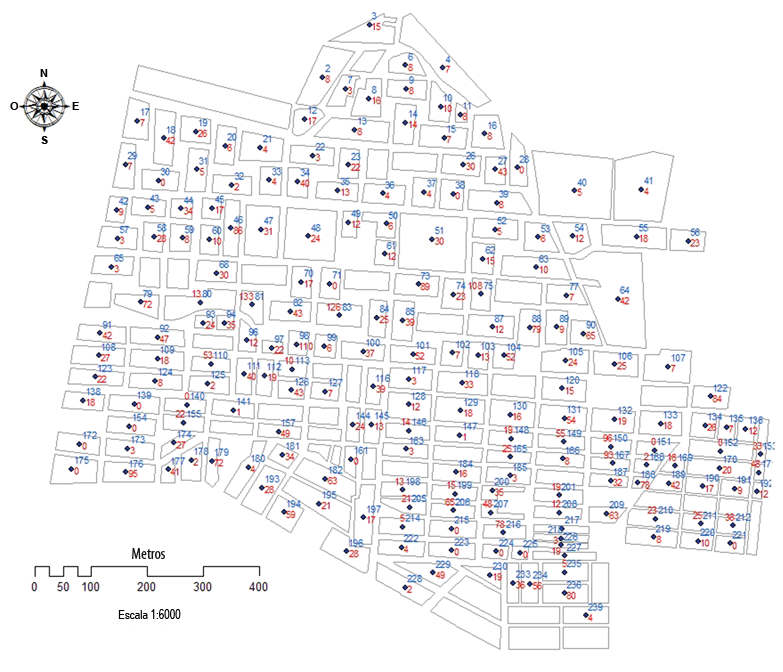
\includegraphics[width=0.7\textwidth]{capitulo-2/graphics/distribucion-puntos-control.png}
\caption{\label{fig:sig-distribucion-puntos-control}Ejemplo de disposición de larvitrampas (azul) y abundancia de larvas (rojo) (Tomado de \cite{NINO2011}).}
\end{figure}

La selección del método de interpolación se realizó teniendo en cuenta el factor humano en la
distribución de los puntos de control. En \cite{villatoro2007comparacion} se realiza una
comparación de los interpoladores IDW y Kriging, donde los autores señalan que el método Kriging
fue más preciso y eficiente que el IDW, aunque la diferencia entre ambos métodos no fue muy amplia.
Sin embargo, cuando el distanciamiento, es muy grande, los variogramas no son posibles de obtener,
entonces el Kriging deja de ser una opción y comparativamente el IDW se perfila como el mejor
\cite{villatoro2007comparacion}. El método seleccionado finalmente fue el IDW, debido que la
distribución del los puntos de control no será perfecta, inclusive, en algunas localidades la
distribución no será de forma uniforme.

\begin{figure}[!htbp]
\centering
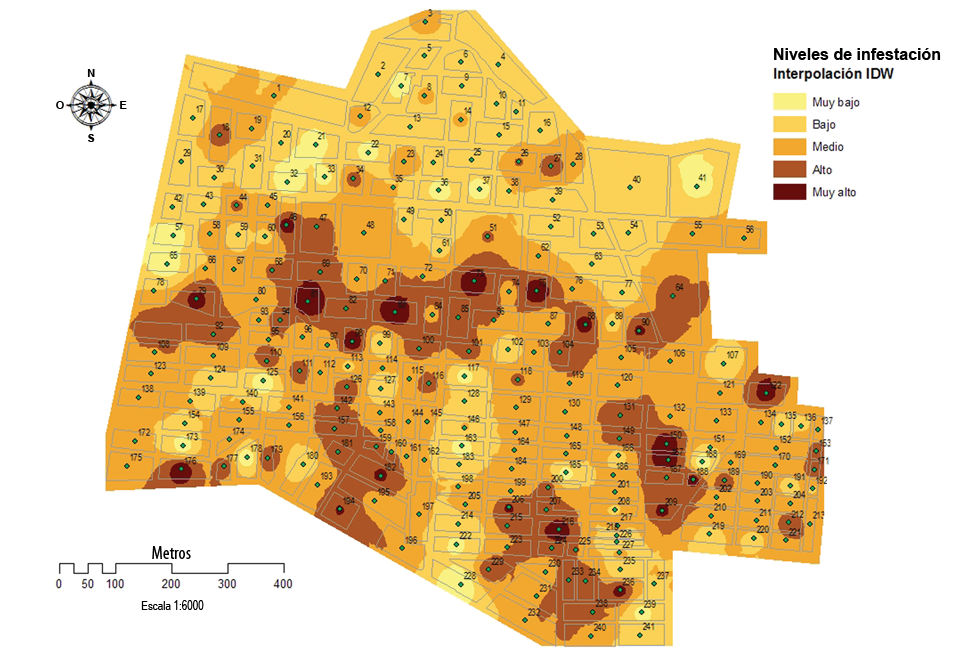
\includegraphics[width=0.7\textwidth]{capitulo-2/graphics/puntos-control-interpolacion.png}
\caption{\label{fig:sig-puntos-control-interpolacion}Ejemplo de mapa de interpolación resultantes (Tomado de \cite{NINO2011}).}
\end{figure}

Los mapas de interpolación resultantes, indican, con mayor detalle que los índices aédicos
tradicionales, los lugares específicos donde sería necesario tomar medidas de prevención y
control de acuerdo al grado de infestación, permitiendo así una mayor racionalización de tiempo y
recursos \cite{NINO2011}.
